
\documentclass{report}
    \title{Statistical Signal Processing \& Inference notes}
    \author{Timothy Chung}
    \date{8/01/24}

\usepackage[a4paper, total={7in, 10in}]{geometry}
\setlength\parindent{0pt}
%=======================PACKAGES FOR NEWCOMMAND CREATION========================
\usepackage{xparse}
%===============================================================================

%=========================PACKAGES FOR USE IN DOCUMENT==========================
\usepackage[dvipsnames]{xcolor}
\usepackage{graphicx, amssymb, amsfonts, amsmath, listings, multirow, hyperref, mathtools, svg, tikz, enumitem, minted, xfrac, multicol}
\usepackage[most]{tcolorbox}
\usepackage[super]{nth}
\usepackage{tabularx}  % for 'X' column type
\usepackage{multirow}  % for multirow cells
\usepackage{pgfplots}
\pgfplotsset{compat=1.17}
\usetikzlibrary{calc}

\usetikzlibrary{shapes.geometric, arrows.meta, positioning}

\tikzset{
    neuron/.style={circle, draw, minimum size=1cm},
    input neuron/.style={neuron, fill=gray!20},
    output neuron/.style={neuron, fill=gray!60},
    activation function/.style={
        rectangle,
        draw,
        minimum size=1cm,
        fill=gray!30,
        path picture={
            % Draw the step function inside the activation function node
            \draw[thick] 
            ($(path picture bounding box.south)+(-0.3cm,0.2cm)$) -- 
            ($(path picture bounding box.south)+(0cm,0.2cm)$) -- 
            ($(path picture bounding box.south)+(0cm,0.7cm)$) -- 
            ($(path picture bounding box.south)+(0.3cm,0.7cm)$);
        }
    },
    arrow label/.style={midway, above}
}


% ======= CUSTOM 
\usepackage{subcaption}
\usepackage{wasysym}

%=================================GLOBAL SETUP==================================
\setitemize{itemsep=0em}
%===============================================================================

%===============================INCLUDE CHAPTERS================================
\newcommand{\addchapter}[1]{\include{#1/#1}}
%===============================================================================

%==============================UNFINISHED SECTION===============================
\newcommand{\unfinished}{\begin{huge} \textcolor{red}{\textbf{UNFINISHED!!!}} \end{huge}}
\newcommand{\toimprove}{\begin{huge} \textcolor{olive}{\textbf{NEEDS IMPROVEMENT!!!}} \end{huge}}
%===============================================================================

%==============================PAGE SPLIT LAYOUTS===============================
\NewDocumentCommand{\twosplit}{O{0.48} O{#1} m m}{
	\begin{minipage}[t]{#1\textwidth}
		#3
	\end{minipage}
	\hfill
	\begin{minipage}[t]{#2\textwidth}
		#4
	\end{minipage}
}
%===============================================================================

%============================SPECIAL COLOURED BOXES=============================

% For term definitions
% \begin{definitionbox}{term}
%	... the term's definition ...
% \end{definitionbox}
\newtcolorbox[auto counter,number within=section]{definitionbox}[2][]{%
	colback=blue!5!white,colframe=blue!75!black,arc=0mm,sharp corners=all,fonttitle=\bfseries,%
	title=#2 \hfill Definition \thetcbcounter #1}

% For term definitions
% \begin{sidenotebox}{cool title}
%	... cool unsassessed/not required info ...
% \end{sidenotebox}
\newtcolorbox[auto counter,number within=section]{sidenotebox}[2][]{%
	colback=black!5!white,colframe=black!75!black,arc=0mm,sharp corners=all,fonttitle=\bfseries,%
	title=#2 \hfill \textit{Extra, Not Assessed} \thetcbcounter #1}
% previously the text was "Extra Fun!"

% For example questions:
% \begin{examplebox}{question name}
%   ... the question ...
%	\tcblower
%   ... the worked answer ...
% \end{examplebox}
\newtcolorbox[auto counter,number within=section]{examplebox}[2][]{%
	colback=orange!5!white,breakable,colframe=orange!75!black,arc=0mm,sharp corners=all,fonttitle=\bfseries,%
	title=#2 \hfill Example Question \thetcbcounter #1}

% For exam questions (no answers):
% \begin{exambox}{1c}{2018}
%   ... the question ...
% \end{exambox}
\newtcolorbox[auto counter,number within=section]{exambox}[3][]{%
	colback=purple!5!white,breakable,colframe=purple!75!black,arc=0mm,sharp corners=all,fonttitle=\bfseries,
	title=Q#2 - #3 \hfill Exam Question \thetcbcounter #1}

% For comments:
% \begin{commentbox}
%   ... the question ...
% \end{commentbox}
 
\newtcolorbox[auto counter,number within=section]{commentbox}[2][]{%
    colback=orange!5!white,
    colframe=orange!95!black, % Darker orange frame
    coltitle=white, % White title text
    arc=0mm,
    sharp corners=all,
    fonttitle=\bfseries,
    title=#2 \hfill
}


 

% For positives/pros 
% \begin{prosbox}
%	... the term's definition ...
% \end{prosbox}
\newtcolorbox[]{prosbox}[1][]{%
	colback=green!5!white,breakable,colframe=green!75!black,leftrule=3mm,arc=0mm,sharp corners=all, #1}

% For negatives/cons 
% \begin{prosbox}
%	... the term's definition ...
% \end{prosbox}
\newtcolorbox[]{consbox}[1][]{%
	colback=red!5!white,breakable,colframe=red!75!black,leftrule=3mm,arc=0mm,sharp corners=all, #1}

% For negatives/cons 
% \begin{tabbox}{consbox}
%	... the term's definition ...
% \end{tabbox}
\newenvironment{tabbox}[2][.8\textwidth]{
	\def\boxtype{#2}
	\begin{\boxtype}
		\begin{center}
			\begin{tabular}{r p{#1}}
				}{
			\end{tabular}
		\end{center}
	\end{\boxtype}
}

% \begin{panoptobox}
%   ... the question ...
% \end{panoptobox}
\newtcolorbox{panoptobox}{enhanced,arc=0mm,breakable,sharp corners=all,colback=gray!5,colframe=gray,leftrule=12mm,detach title,%
	underlay unbroken and first={\node[below,text=black,anchor=east] at (interior.base west) {\includegraphics[width=11mm]{../common/images/panopto_logo.png}};}}

\newcommand{\lectlink}[2]{
	\begin{panoptobox}
		\textbf{\href{#1}{#2}}
	\end{panoptobox}
}
%===============================================================================
\newcommand{\infer}[2]{\cfrac{#1}{#2}}
\newcommand{\infers}[3]{\cfrac{#1}{#2}(#3)}

\newcommand{\ninfer}[3]{(\text{#1}):\cfrac{#2}{#3}}
\newcommand{\ninfers}[4]{(\text{#1}):\cfrac{#2}{#3}(#4)}
\newcommand{\ainfer}[3]{\cfrac{#2}{#3}(\text{#1})}

\newcommand{\mllet}[2]{\text{let } #1 \text{ in } #2}
\newcommand{\mlfix}[2]{\text{fix } #1 . #2}

\newcommand{\hc}{\mathcal{H}}
\newcommand{\cov}{\text{Cov}}
\newcommand{\E}{\text{E}}
\newcommand{\var}{\text{Var}}
\newcommand{\mb}{\mathbf}
\newcommand{\est}{\hat{\theta}}
\newcommand{\p}{\theta}



\begin{document}
\include{titlepage/titlepage}

\begin{titlepage}
    \centering
    \vspace*{1cm}
    \Huge
    \textbf{ELEC60002 Statistical Signal Processing and Inference} \\
    \vspace{1cm}
    \Large
    Timothy Chung \\
    \vspace{1cm}
    Spring 2024 \\
    \vfill
\end{titlepage}

\setcounter{tocdepth}{1}
\tableofcontents
\newpage
\setcounter{chapter}{-1}
\chapter{Foreword}
The notes are intended to be a gentle introductory supplement to the well-documented course notes, and not a full replacement with all the bells and whistles (e.g. real life use-cases, mathematical examples). The full notes are available on Professor Danilo Mandic's website \href{https://www.commsp.ee.ic.ac.uk/~mandic/courses.htm}{here.}\\


Thus, a better title for this document would be `Elements of Statistical Signal Processing and Inference'.

\sn{On The Rigour of A Random Variable}{
For the beginning of this module, a random variable $X$ is considered to be a function from a sample space $\Omega$ to the unit interval $[0, 1]$. However, in Lectures 6 and 7, we use the full definition of a random variable, which is a measurable function from a sample probability space $(\Omega)$ to a measurable space $(E, \varepsilon)$, involving the concept of $\sigma$-algebras and measure spaces. \bigskip

When the sample space is a continuous space, the function $p$ is a \textbf{probability density function} (PDF). When the sample space is a discrete space, the function $p$ is a \textbf{probability mass function} (PMF).
} 


\marginnote[-60pt]{We will introduce measure theory later.}





\section{Brief Probability Theory Review}

$x$ is a sample from a random variable $X$. 

\noindent $P(X=x)$ refers to probability that the random variable $X$ takes on the value $x$.

\subsection{Probability Density Function (PDF)}
\begin{marginfigure}[100pt]
    \centering
    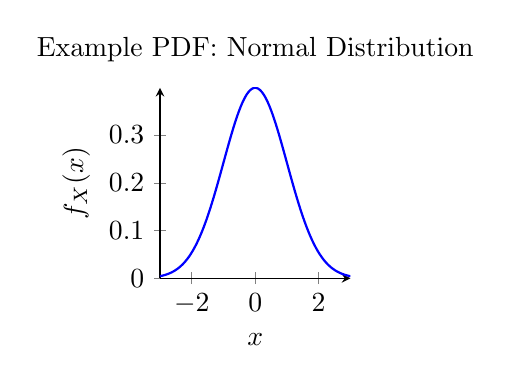
\begin{tikzpicture}
        \begin{axis}[
            width=4cm,
            height=4cm,
            xlabel={$x$},
            ylabel={$f_X(x)$},
            domain=-3:3,
            samples=100,
            axis lines=left,
            ymin=0,
            legend pos=north east,
            title={Example PDF: Normal Distribution}
        ]
        \addplot[blue, thick] {exp(-x^2 / 2) / sqrt(2 * pi)};
        \end{axis}
    \end{tikzpicture}
    \caption{Probability Density Function of a standard normal distribution}
\end{marginfigure}

The Probability Density Function (PDF) of a continuous random variable \(X\) is a function \(f_X(x)\) that describes the relative likelihood for this random variable to take on a given value. The PDF has the following properties:
\begin{itemize}
    \item \(f_X(x) \geq 0\) for all \(x\).
    \item \(\int_{-\infty}^{\infty} f_X(x) \, dx = 1\).
\end{itemize}

Mathematically, the PDF is defined such that the probability that \(X\) lies within a particular interval \([a, b]\) is given by:
\[
P(a \leq X \leq b) = \int_{a}^{b} f_X(x) \, dx.
\]


\subsection{Cumulative Distribution Function (CDF)}
\begin{marginfigure}[50pt]
    \centering
    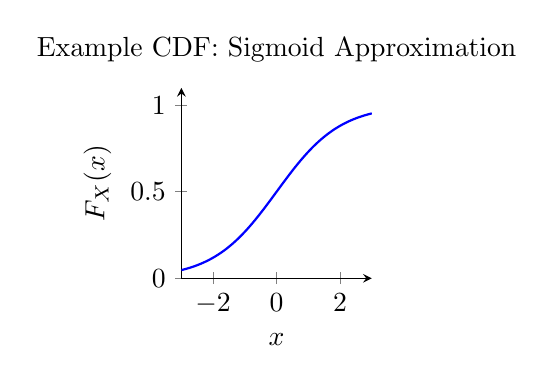
\begin{tikzpicture}
        \begin{axis}[
          width=4cm,
          height=4cm,
            xlabel={$x$},
            ylabel={$F_X(x)$},
            domain=-3:3,
            samples=100,
            axis lines=left,
            ymin=0, ymax=1.1,
            legend pos=south east,
            title={Example CDF: Sigmoid Approximation}
        ]
        \addplot[blue, thick] {1 / (1 + exp(-x))};
        \end{axis}
    \end{tikzpicture}
    \caption{Cumulative Distribution Function}
\end{marginfigure}

The Cumulative Distribution Function (CDF) of a continuous random variable \(X\) is a function \(F_X(x)\) that describes the probability that \(X\) will take a value less than or equal to \(x\). It is defined as:
\[
F_X(x) = P(X \leq x) = \int_{-\infty}^{x} f_X(t) \, dt.
\]

The CDF has the following properties:
\begin{itemize}
    \item \(0 \leq F_X(x) \leq 1\) for all \(x\).
    \item \(F_X(x)\) is a non-decreasing function.
    \item \(\lim_{x \to -\infty} F_X(x) = 0\).
    \item \(\lim_{x \to \infty} F_X(x) = 1\).
\end{itemize}


\subsection{Dealing with Data (Single-Feature)}

In Machine Learning (ML), we often deal with large datasets from which we aim to extract meaningful insights. It is useful to model these data points as random variables:
\[
\{x_1, x_2, \ldots, x_N\}
\]


\noindent We typically model these samples as random variables:

\[
\{x_1 \sim X_1, x_2 \sim X_2, \ldots, x_N \sim X_N\}
\]

\subsection{Vectors of Random Variables}

When dealing with joint random variables, we often represent them as vectors:

\[
\mathbf{X} = (X_1, X_2, X_3) \quad \text{with joint distribution} \quad p_{X_1, X_2, X_3}(x_1, x_2, x_3)
\]

\noindent For a vector of random variables \(\mathbf{X}\) in \( \mathbb{R}^3 \), the joint probability density function is denoted as:

\[
p_{\mathbf{X}}(\mathbf{x}) \quad \text{where} \quad \mathbf{X} \in \mathbb{R}^3
\]
\noindent 
If these are input observations, they are often referred to as "feature vectors."

\subsection{Distinct Random Variables}

We model samples as distinct random variables \sidenote[][-20pt]{\textbf{Why should we model these as distinct random variables? Aren't they all the same thing?} \smallskip

\noindent Despite being identically distributed, distinct random variables allow for capturing dependencies and interactions between different samples.
}:\bigskip

\[
\{x_1 \sim X_1, x_2 \sim X_2, \ldots, x_N \sim X_N\}
\]


\section{Independent and Identically Distributed (i.i.d.) Random Variables}

\marginnote[-50pt]{    \textbf{Why do we model samples as distinct random variables?}

\begin{enumerate}
    \item By treating each sample as a distinct variable, we assume samples are i.i.d, allowing every sample to contribute independently to the likelihood of oberving the data given the model prarameters – so every sample provides unique information to estimate the parameters of the underlying distribution. If we treated all samples as a single random variable, we would lose the granularity of information, leading to a poorer estimate.
    \item Treating samples as distinct allows us to study and model the relationships and dependencies between them.
    \item The assumption of i.i.d follows many results in probability and statistics, such as the Central Limit Theorem, which states that the sum of a large number of i.i.d. random variables is approximately normally distributed. It is also an assumed requirement for a model to generalise. The assumption simplifies the analysis and derivation process, allowing us to use techniques like maximum likelihood estimation (MLE) and empirical risk minimization (ERM).
\end{enumerate}
    }
\subsection{Independence of Random Variables}

Independence refers to the idea that the values or outcomes of one observation in a dataset do not depend on or influence the values of any other observation.\\

For the set of random variables $X_1, X_2, \ldots X_n$, for the collection \[\{x_1 \sim X_1, x_2 \sim X_2, \ldots, x_N \sim X_N\}\]

\noindent we often assume independence, for any subset of observations \(\{X_{i1}, X_{i2}, \ldots, X_{ik}\}\) where \(i_1, i_2, \ldots, i_k \in \{1, 2, \ldots, N\}\), the joint distribution factorises:

\begin{equation}
P(X_{i_1} = x_{i_1}, \ldots, X_{i_k} = x_{i_k}) = P(X_{i_1} = x_{i_1}) \cdot \ldots \cdot P(X_{i_k} = x_{i_k})
\end{equation}

\hl{The joint distribution of the subset is the product of the marginal distributions of the individual random variables.} \bigskip

\textbf{Independence:} The occurrence of any event does not affect the occurrence of others. This is a crucial assumption in many ML models that we will see the usefulness of as early as the next lecture.

\subsection{Identically Distributed Random Variables}

The "identically distributed" part of i.i.d. refers to the idea that all random variables in the sample follow the same probability distribution. That is, they share the same probability density function (pdf) or probability mass function (pmf), depending on whether the data is continuous or discrete. If the set of random variables \(\{X_1, X_2, \ldots, X_n\}\) are identically distributed, then:





\begin{equation}
    f_{X_1}(x) = f_{X_2}(x) = \ldots = f_{X_n}(x) = f_{X}(x)
\end{equation}

\begin{equation}
F_{X_1}(x) = F_{X_2}(x) = \ldots = F_{X_n}(x) = F_{X}(x)
\end{equation}

\noindent This implies that the cumulative distribution function (CDF) is the same for all these random variables.


\section{Statistical Modelling as Curve Fitting}

Machine learning and statistics have significant overlap, and so most concepts studied in this module can be cast as statistical modelling. Consider our random variables:

\begin{equation}
\{x_1 \sim X_1, x_2 \sim X_2, \ldots, x_N \sim X_N\}
\end{equation}

\noindent These random variables can be modelled to fit certain curves that represent the underlying data distribution. 

\subsection{Assumption about the Model}

To proceed with statistical modelling, we make an assumption about the form of the model:

\begin{equation}
P_X(x) \approx \mathcal{N}(x; \theta) \quad \theta := (\mu, \sigma)
\end{equation}

Here, \(P_X(x)\) is approximated by a normal distribution \(\mathcal{N}(x; \theta)\), where \(\theta\) represents the parameters of the distribution, namely the mean \(\mu\) and the standard deviation \(\sigma\). This assumption simplifies the process of modelling the data.

\subsection{Fitting the Model}

The next step is to fit the model to the data. This involves finding the parameter values \(\theta\) that maximize the probability of observing the given data. Mathematically, this is expressed as:

\begin{equation}
\arg \max_{\theta} P(x_1, \ldots, x_N \mid \theta)
\end{equation}

In other words, we adjust the parameters \(\mu\) and \(\sigma\) so that the assumed model best fits the observed data. This process is known as maximum likelihood estimation (MLE).\\











\section{Discrete Random Variables}


\subsection{Bernoulli and Multinoulli Distributions}
\textbf{Bernoulli Distribution:} Outcome with two values (e.g., heads or tails).
\begin{itemize}
    \item Parameter: \(\theta\).
    \item Probabilities: \(P(X = 0) = 1 - \theta\), \(P(X = 1) = \theta\).
\end{itemize}

\textbf{Multinoulli Distribution:} Describes a scenario with multiple possible outcomes, extending the Bernoulli distribution to more than two outcomes.
\begin{itemize}
    \item Parameter: \(\bm{\theta} \in \mathbb{R}^s\) where each \(\theta_i\) represents the probability of the \(i\)-th outcome, and \(\sum_{i=0}^{s-1} \theta_i = 1\).
    \item Probabilities: \(P(X = i) = \theta_i\) for \(i = 0, 1, \ldots, s-1\).
\end{itemize}

\subsection{Binomial and Multinomial Distributions}
\textbf{Binomial Distribution:} \(X \sim \text{Bin}(n, \theta)\).
\begin{itemize}
    \item Probability Mass Function (p.m.f):
    \[
    \text{Bin}(k \mid n, \theta) := \binom{n}{k} \theta^k (1 - \theta)^{n-k}
    \]
    \item Binomial Coefficient:
    \[
    \binom{n}{k} = \frac{n!}{(n - k)!k!}
    \]
    \item Mean: \(n\theta\).
    \item Variance: \(n\theta(1 - \theta)\).
\end{itemize}

\textbf{Multinomial Distribution:} Generalises the binomial distribution for more than two outcomes. It models the probabilities of counts among multiple categories in \(n\) independent trials.
\begin{itemize}
    \item Parameters: \(n\) (number of trials) and \(\boldsymbol{\theta} = (\theta_1, \theta_2, \ldots, \theta_K)\) where \(\theta_i\) is the probability of the \(i\)-th category and \(\sum_{i=1}^{K} \theta_i = 1\).
    \item Probability Mass Function (p.m.f):
    \[
    \text{Mu}(\mathbf{x} \mid n, \boldsymbol{\theta}) := \binom{n}{x_1, x_2, \ldots, x_K} \prod_{j=1}^{K} \theta_j^{x_j}
    \]
    where \(\mathbf{x} = (x_1, x_2, \ldots, x_K)\) represents the count of occurrences for each category.
    \item Multinomial Coefficient:
    \[
    \binom{n}{x_1, x_2, \ldots, x_K} = \frac{n!}{x_1! x_2! \cdots x_K!}
    \]
    \item Mean for each category \(i\): \(\mathbb{E}[X_i] = n\theta_i\).
    \item Variance for each category \(i\): \(\text{Var}(X_i) = n\theta_i(1 - \theta_i)\).
    \item Covariance between categories \(i\) and \(j\): \(\text{Cov}(X_i, X_j) = -n\theta_i\theta_j\).
\end{itemize}


\subsection{Empirical Distribution}
\defb{Empirical Distribution}{
Based on observation or experience rather than theory or pure logic.
}


\begin{intuitbox}{Empirical Distribution}
    

    Practically, we do not have access to an infinite amount of data, but we have instead a small fraction of it, a sample, to infer any insights from it. In the case of discrete random variables, we use probability mass functions, which is straightforward, but we are interested in probability density functions for continuous random variables, because to model the true distribution, we would need an infinite number of samples. \bigskip

    Thus, our goal is to approximate the true PDF from a given data set using finite samples. The transformation from discrete to continuous is done with the Dirac delta function.\\ \bigskip

    A Dirac delta function is interestingly helpful because:
    \[
    \int_{-\infty}^{\infty} \delta(x) \, dx = 1
    \]

    We can then have multiple Dirac delta functions to represent the empirical distribution of a data set, but scaled down by a factor equivalent to the total number of data points to ensure the area under the curve is 1.\\

    \begin{center}
        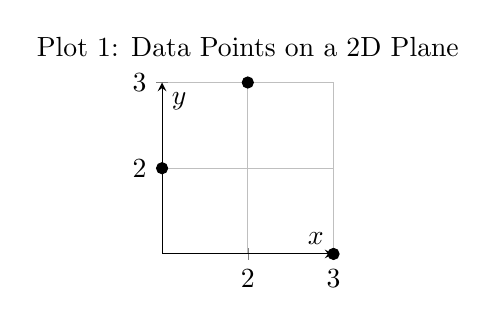
\begin{tikzpicture}
            \begin{axis}[
                title={Plot 1: Data Points on a 2D Plane},
                xlabel={$x$},
                ylabel={$y$},
                axis lines=middle,
                grid=major,
                width=0.31\textwidth,
                height=0.31\textwidth,
                xtick={1, 2, 3},
                ytick={0, 1, 2, 3}
            ]
                \addplot[only marks, mark=*, mark size=2pt] coordinates {(1,2) (2,3) (3,1)};
            \end{axis}
        \end{tikzpicture}
        \hspace{1cm}
        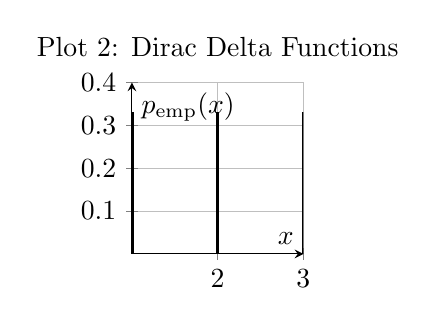
\begin{tikzpicture}
            \begin{axis}[
                title={Plot 2: Dirac Delta Functions},
                xlabel={$x$},
                ylabel={$p_{\text{emp}}(x)$},
                axis lines=middle,
                grid=major,
                width=0.31\textwidth,
                height=0.31\textwidth,
                ymin=0, ymax=0.4,
                xtick={1,2,3},
                ytick={0,0.1,0.2,0.3,0.4}
            ]
                \addplot[very thick] coordinates {(1,0) (1,0.33)};
                \addplot[very thick] coordinates {(2,0) (2,0.33)};
                \addplot[very thick] coordinates {(3,0) (3,0.33)};
            \end{axis}
        \end{tikzpicture}
        \hspace{1cm}
        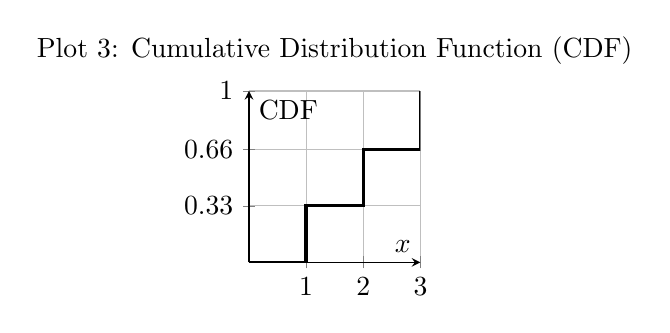
\begin{tikzpicture}
            \begin{axis}[
                title={Plot 3: Cumulative Distribution Function (CDF)},
                xlabel={$x$},
                ylabel={CDF},
                axis lines=middle,
                grid=major,
                width=0.31\textwidth,
                height=0.31\textwidth,
                ymin=0, ymax=1,
                xtick={1, 2, 3},
                ytick={0, 0.33, 0.66, 1}
            ]
                \addplot[very thick] coordinates {(0,0) (1,0) (1,0.33) (2,0.33) (2,0.66) (3,0.66) (3,1)};
            \end{axis}
        \end{tikzpicture}
    \end{center}
    
\end{intuitbox}

\marginnote[-120pt]{    \refsb{Recommended Viewing}{
  \href{https://www.youtube.com/watch?v=7f3YFT7bsmg}{Lecture on Empirical Distribution}\smallskip

  Empirical Statistics: When you compute statistics from a dataset, you're really computing statistics for its empirical distribution.\smallskip

  A dataset is, in essence, a distribution.
}}


\textbf{Empirical Distribution:} Suppose we have a set of data samples 

$$D = \{x^{(1)}, x^{(2)}, \ldots, x^{(N)}\} $$

derived from a random variable \(X\). We can approximate the distribution of \(X\) using a set of delta functions on these samples:
% Represents the distribution of a given data set \(D = \{x^{(1)}, \ldots, x^{(N)}\}\).
\begin{itemize}
    \item For a given data set \(D\), the empirical distribution \(p_{\text{emp}}(x)\) is defined as:
    \[
    p_{\text{emp}}(x) := \frac{1}{N} \sum_{i=1}^N \delta_{x_i}(x)
    \]
    where \(\delta_{x_i}(x)\) is the Dirac measure centred at \(x_i\).
    \item \textbf{Dirac Measure:} \(\delta_{x_i}(x)\) is a function that is 1 if \(x = x_i\) and 0 otherwise. Formally, it is defined as:
    \[
    \delta_{x_i}(x) = \begin{cases} 
    1, & \text{if } x = x_i \\
    0, & \text{if } x \neq x_i 
    \end{cases}
    \]
    \item Explanation: The empirical distribution assigns equal probability \( \frac{1}{N} \) to each observed data point \(x_i\). It is a discrete distribution that places mass only on the observed data points.
    \item In general, one can associate weights with each element of the empirical distribution, i.e., \(p_{\text{emp}}(x) = \frac{1}{N} \sum_{i=1}^N w_i \delta_{x_i}(x)\) as long as each \( 0 \leq w_i \leq 1 \) and \( \sum_{i=1}^N w_i = 1 \).
\end{itemize}

\section{Continuous Random Variables}

\subsection{Gaussian (Normal) Distribution}
\textbf{Probability Density Function (p.d.f):}
\begin{itemize}
    \item Formula: \[
    N(x \mid \mu, \sigma^2) = \frac{1}{\sqrt{2\pi\sigma^2}} \exp\left(-\frac{(x - \mu)^2}{2\sigma^2}\right)
    \]
    \item Mean: \(\mu = \mathbb{E}[X]\).
    \item Variance: \(\sigma^2 = \text{Var}[X]\).
    \item Standard Normal Distribution: \(X \sim N(0, 1)\).
    \item Precision: \(\lambda = \frac{1}{\sigma^2}\).
\end{itemize}
\textbf{Cumulative Distribution Function (CDF):}
\begin{itemize}
    \item Formula: \[
    \Phi(x; \mu, \sigma^2) = \int_{-\infty}^x N(z; \mu, \sigma^2) \, dz
    \]
    \item In terms of the error function (erf):
        \[
        \Phi(x; \mu, \sigma^2) = \frac{1}{2} \left[1 + \text{erf}\left(\frac{z}{\sqrt{2}}\right)\right]
        \]
        where \(z = \frac{x - \mu}{\sigma}\) and
        \[
        \text{erf}(x) = \frac{1}{\sqrt{\pi}} \int_0^x \exp(-t^2) \, dt
        \]
\end{itemize}


\section{Viewing Data}

\begin{itemize}
    \item Data (coordinates) Perspective (Design Matrix) 
    \item Set Perspective
    \begin{itemize}
        \item Combination invariant
        \item Allows for natural language....??
    \end{itemize}
    \item Empirical Distribution Perspective
    \begin{itemize}
        \item i.i.d
    \end{itemize}
\end{itemize}


\section{Example Scene: Self-Driving Car}
\sn{Notation and Gotchas}{
    The lecture use $x_i$ to denote the $i$-th feature, and $x^{(i)}$ to denote the $i$-th data point. The slides however seem to denote $x_i$ as the $i$-th data point. The notes follow the former convention.\\

    Also, it is generally assumed that in a classification problem, the classes are distinct and mutually exclusive, so an image is either a dog or a cat (multi-class classfication) but not a combination of both (multi-label classification). The course focuses on the former convention.

}
Take a case of the self-driving car. There are several facets:
\begin{enumerate}
    \item \textbf{Object Recognition: }identifying objects in the scene (classification)
          \begin{itemize}[noitemsep]
              \item An image is a 2D array of pixel values. For a colour image, each pixel has 3 values (RGB).
              \item \textbf{Input:}
                    \begin{equation}
                        x \in \mathbb{R}^{H \times W \times C}
                    \end{equation}
                    where $H$ is height, $W$ is width, and $C$ is the number of channels (e.g. 3 for RGB)
              \item \textbf{Output:} We would like to detect if something is a background, another vehicle, the ground level, or a pedestrian. Let's say there are $m$ outcomes, making this a \textbf{classification problem}. Naively, let
                    $y \in \mathbb{R}^m$. However, these numbers are just arbitrary i.e. raw scores. It would make more sense to refine the output to a probability distribution over the $m$ classes: \\
                    \begin{equation}
                        y \in \Delta^m \quad \text{where }\sum_{i=1}^{m} y_i = 1
                    \end{equation}
                    Where the $\Delta^m$ is the $m$-simplex, where the sum of all elements is 1. This provides a measure of ``confidence'' in the prediction. Example: To choose between four classes: [Vehicle, Pedestrian, Road, Background], the output could be $[0.1, 0.7, 0.1, 0.1]$. This means the model is 70\% confident that the object is a pedestrian.
              \item \textbf{Our objective is to learn a function:}
                    \begin{equation}
                        f^\theta : x^{(i)} \mapsto y^{(i)} \quad \text{where } \theta \text{ are model parameters}, x^{(i)} \in \mathbb{R}^{H \times W \times C}, y^{(i)} \in \Delta^m
                    \end{equation}
                    \begin{marginfigure}
                        \centering
                        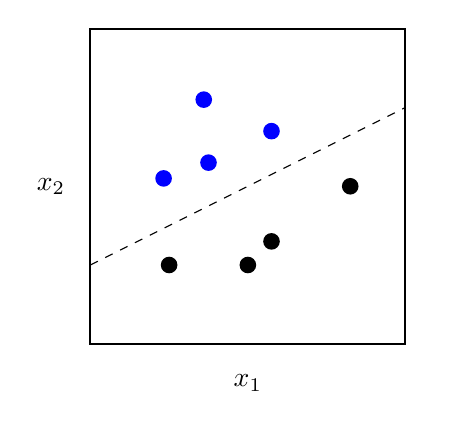
\begin{tikzpicture}
                            % Draw the outer square
                            \draw[thick, black] (0,0) rectangle (4,4);
                            % Draw the blue points
                            \fill[blue] (1.44,3.1) circle (3pt);
                            \fill[blue] (1.5,2.3) circle (3pt);
                            \fill[blue] (0.93,2.1) circle (3pt);
                            \fill[blue] (2.3,2.7) circle (3pt);
                            % Draw the black points
                            \fill[black] (3.3,2) circle (3pt);
                            \fill[black] (2.3,1.3) circle (3pt);
                            \fill[black] (2,1) circle (3pt);
                            \fill[black] (1,1) circle (3pt);
                            % Labels for the axes
                            \node at (2,-0.5) {$x_1$};
                            \node at (-0.5,2) {$x_2$};
                            % Dashed separator
                            \draw[dashed] (0,1)--(4,3) node[right] {};
                        \end{tikzpicture}
                        \caption{Simplified example for $f^\theta$}
                        \label{fig:1_classification}
                    \end{marginfigure}
                    A simplified example for $f^\theta$ is shown in Figure \ref{fig:1_classification}. Ideally, we want a separator that separates the input space into $m$ distinct regions according to observed data.

              \item \textbf{Data Formalisation (1): }We can view our dataset as a set of $N$ pairs where $x^{(i)}$ is an image and $y^{(i)}$ is the corresponding label. More neatly put,
                    \begin{equation}
                        \mathcal{D} = \{(x^{(i)}, y^{(i)})\}_{i=1}^{N}, \quad x^{(i)} \in \mathbb{R}^{H \times W \times C}, y^{(i)} \in \Delta^m
                    \end{equation}
              \item \textbf{Data Formalisation (2): } We could also view the dataset as an empirical distribution over the data space like in Figure \ref{fig:1_distribution}:
                    \begin{equation}
                        \mathcal{D} = \{x^{(i)}, y^{(i)}\}_{i=1}^{N} \sim p_{\text{data}}(x, y)
                    \end{equation}
                    \begin{marginfigure}
                        \centering
                        \begin{tikzpicture}
                            \begin{axis}[
                                view={0}{90},
                                axis on top,
                                enlargelimits=false,
                                colormap/viridis,
                                xlabel={$x_1$},
                                ylabel={$x_2$},
                                % colorbar,
                                samples=50, % Adjusting the sample size
                                domain=-5:5,
                                width=2in,
                                height=2in
                            ]
                            
                            % First contour group
                            \addplot3[
                                contour gnuplot={
                                    levels={0.25, 0.4, 0.55, 0.65, 0.79, 1, 1.25, 1.5}
                                }
                            ]
                            {exp(-((x)^2 + (1.4*y)^2))};
                    
                            % Second contour group
                            \addplot3[
                                contour gnuplot={
                                    levels={0.25, 0.4, 0.55, 0.65, 0.79, 1, 1.25, 1.5}
                                }
                            ]
                            {exp(-((2*x+2)^2 + (y+2)^2))};
                            
                            \end{axis}
                        \end{tikzpicture}
                        \caption{Viewing the dataset as an empirical distribution}
                        \label{fig:1_distribution}
                    \end{marginfigure}
                    



          \end{itemize}
          \item \textbf{Route Planning:} 
          We aim to predict the optimal path, where the prediction function \( f^\theta \) takes spatial data and environmental conditions as input and outputs a route (either as a series of decisions or waypoints).
          \begin{itemize}[noitemsep]
              \item \textbf{Input:}
              \begin{equation}
                  x \in \mathbb{R}^{n}
              \end{equation}
              where \( x \) could represent a vector of features including road conditions, traffic density, and start/end coordinates.
              
              \item \textbf{Output:} 
              A route \( y \), represented either as a classification over a set of discrete routes, or as continuous waypoints:
              \begin{equation}
                  f^\theta : x \mapsto y
              \end{equation}
              Here, \( y \in \mathbb{R}^m \) for \( m \) possible waypoints (or classes, if we use a discrete route classification).
          \end{itemize}
          The objective is to minimise the difference between predicted and actual routes, defined as a suitable loss function \( \mathcal{L}(f^\theta(x), y) \).

    \item \textbf{Speed Control:} 
    \sn{Ordinal Regression here?}{To update}
          In this problem, we predict the optimal driving speed, and \( f^\theta \) models the relationship between environmental and driving conditions and speed.
          \begin{itemize}[noitemsep]
              \item \textbf{Input:} 
              \begin{equation}
                  x \in \mathbb{R}^p
              \end{equation}
              where \( x \) represents features such as current speed, distance to obstacles, road surface, and weather conditions.
              
              \item \textbf{Output:} 
              A continuous speed value \( y \in \mathbb{R} \):
              \begin{equation}
                  f^\theta : x \mapsto y
              \end{equation}
              where \( y \) is the predicted speed. This is a regression problem, so the goal is to minimise the squared error:
              \begin{equation}
                  \mathcal{L}(\theta) = \frac{1}{N} \sum_{i=1}^{N} (f^\theta(x^{(i)}) - y^{(i)})^2
              \end{equation}
          \end{itemize}

    \item \textbf{Steering Angle Prediction:}
          Steering angle prediction aims to output a continuous angle based on the driving conditions, making it a regression problem.
          \begin{itemize}[noitemsep]
              \item \textbf{Input:}
              \begin{equation}
                  x \in \mathbb{R}^q
              \end{equation}
              where \( x \) could represent lane position, vehicle surroundings, and road curvature.
              
              \item \textbf{Output:} 
              The predicted steering angle \( y \in \mathbb{R} \):
              \begin{equation}
                  f^\theta : x \mapsto y
              \end{equation}
              This is also a regression task, and the loss function could again be the squared error:
              \begin{equation}
                  \mathcal{L}(\theta) = \frac{1}{N} \sum_{i=1}^{N} (f^\theta(x^{(i)}) - y^{(i)})^2
              \end{equation}
          \end{itemize}
\end{enumerate}

\section{Mathematics of Linear Models}

Linear models are fundamental in statistics and supervised machine learning. They can:
\begin{itemize}[noitemsep]
    \item Handle linear relationships.
    \item Be augmented with kernels or basis functions to model non-linear relationships.
    \item Provide analytical tractability for studying concepts like convergence, probabilistic modelling, and overfitting.
\end{itemize}
This section introduces the linear regression model.

\subsection{Linear Regression Model}

Linear regression involves performing regression with a linear model in a supervised setting. Given a dataset \(\mathcal{D}\) consisting of input-output pairs \((\bm{x}^{(i)}, y^{(i)})\) for \(i = 1, \ldots, N\):
\begin{itemize}[noitemsep]
    \item \(\bm{x} \in \mathbb{R}^n\) represents the input features.
    \item \(y \in \mathbb{R}\) represents the output or target variable.
    \item Assume a domain \(\mathbb{R}^n\) and a one-dimensional co-domain.
    \item Model: \(f(\bm{x}) = \bm{x}^\top \bm{\theta}\).
    \item Noise: \(\epsilon \sim \mathcal{N}(0, \sigma^2)\).
\end{itemize}
The full model is:
\[
\hat{y}^{(i)} = \bm{x}^{(i)\top} \bm{\theta} + \epsilon
\]

The objective is to find \(\bm{\theta}\) such that \(\hat{y}^{(i)} \approx y^{(i)}\). In other words, we want to find a set of parameters \(\bm{\theta}\) that best explains the relationship between the input features \(\bm{x}\) and the target variable \(y\). This means minimising the difference between the predicted values \(\hat{y}\) and the actual values \(y\).\bigskip

\textbf{Conventions and Notations:}
\begin{itemize}[noitemsep]
    \item Vectors \(\bm{x} \in \mathbb{R}^n\) are column vectors, written as \(n \times 1\) matrices.
    \item \(\bm{x}^\top\) (x transpose) swaps rows and columns of \(\bm{x}\), resulting in a \(1 \times n\) row vector.
\end{itemize}




\begin{referencebox}{Lecture Reading}
    Chapter 1-2 of Kevin Murphy's \textit{Machine Learning: A Probabilistic Perspective}. Chapter 1.4 was not covered, but may be of interest
\end{referencebox}





\chapter{Linear Stochastic Models}

\section{Objectives}
\begin{itemize}
    \item Introduce linear stochastic models for real world data
    \item Understand stochastic processes for noise
    \item ARMA models, partial correlations, and optimal model order selection criteria (MDL, AIC,...)
\end{itemize}
\begin{theorembox}{Wold's Decomposition Theorem}

Any covariance-stationary time series can be decomposed into two different parts: \textbf{deterministic} and \textbf{stochastic}.\\

Let $w$ denote a white process, $x_r[n]$ a regular random process, and $x_p[n]$ a predictable process such that $x_r[n]\perp x_p[n]$.

\begin{align}
x[n]&=x_p[n]+x_r[n]\\
&=x_p[n]+\sum_{j=1}^qb_jw[n-j]
\end{align}

The condition requires $\E[x_r[m]x_p[n]]=0$.

\end{theorembox}

\begin{definitionbox}{Deterministic vs Stochastic}
    \begin{itemize}
        \item Deterministic means a component can be precisely described by an equation without any randomness, following a predictable pattern that can be determined exactly for any point in time, e.g. a sine wave.
        \item Stochastic means a component described by a random process. It cannot be described by a simple equation but can be represented using a probability distribution, such as WGN (Filtered White Gaussian) noise.
    \end{itemize}
\end{definitionbox}

\section{WSS Process}
A WSS process has two conditions:
\begin{enumerate}
    \item The mean of the process is constant for all time, i.e., \( \E[X_t] = \mu \) for all \( t \), where \( \mu \) is a constant.
    \item The autocovariance function \( R_x(t, t+\tau) = \text{Cov}(X_t, X_{t+\tau}) \) depends only on the time lag \( \tau \) and not on time \( t \) itself, i.e., \( R_x(t, t+\tau) = R_x(\tau) \).
\end{enumerate}

The general form for the power spectrum of a WSS process is 
\begin{equation}
P_x(e^{j\omega})=\sum_{k=1}^N\alpha_k\delta(\omega-\omega_k)+P_{x_r}(e^{j\omega})
\end{equation}

\begin{definitionbox}{Linearly Deterministic Process}
    A covariance-stationary process is called linearly deterministic if $p(x[n]\mid x[n-1],x[n-2],\ldots)=x[n].$ It can be predicted correctly with zero error if we know its entire past data $x[n-1],x[n-2],\ldots$
\end{definitionbox}

\section{ARMA Models}
ARMA models are a linear stochastic model.\\

Autoregressive (AR) filters use an all-pole system and Moving Average (MA) filters use an all-zero system. An Autoregressive Moving Average (ARMA) filter utilises both poles and zeroes.\\

In ARMA modelling we filter white noise $w[n]$ with a causal linear shift-invariant filter (transfer function $H[z]$ that has $p$ poles and  $q$ zeroes. 

\begin{equation}\label{eq:ARMA}
    X(z)=H(z)W(z)\quad\Rightarrow\quad H(z)=\frac{B_q(z)}{A_p(z)}=\frac{\sum_{k=0}^qb_kz^{-k}}{1+\sum_{k=1}^pa_kz^{-k}}
\end{equation}

If our filter is WSS, then $x[n]$ is WSS as well. To show this, multiply both sides of Equation \ref{eq:ARMA} by $x[n-k]$ can calulating expectation, we have

\begin{equation}
    r_{xx}(k)=\underbrace{\sum_{l=1}^pa_lr_{xx}(k-l)}_{\color{red}{\text{easy to calculate}}}+\underbrace{\sum_{l=0}^qb_lr_{xw}(k-l)}_{\color{red}{\text{can be complicated}}}
\end{equation}

Note that since $X(z) = H(z)W(z)$ the random processes $x[n]$ and $w[n]$ are related by a linear difference equation with constant coefficients. This is 

\begin{equation}
    \begin{aligned}\mathrm{ARMA(p,q)}=H(z)=&\frac{B(z)}{A(z)}=\frac{\sum_{k=0}^qb_kz^{-k}}{1+\sum_{k=1}^pa_kz^{-k}}\\x[n]=&\underbrace{\sum_{l=1}^pa_lx[n-l]}_{\text{autoregressive}}+\underbrace{\sum_{l=0}^qb_lw[n-l]}_{\text{moving average}}\end{aligned}
\end{equation}

Note that for $H(z)$, coefficients must be absolutely summable. For the process to be stationary, $\sum_{j=0}^\infty|b_j|<\infty$, and for it to be invertible, $\sum_{j=0}^\infty|a_j|<\infty$.


\section{AR Processes}
An autoregressive process of order p, denoted by $AR(p)$ can be described by:

\begin{align}
    x[n] =& a_1x[n-1] + a_2x[n-2]+ \ldots + a_p[n-p] + w[n] \\=&\sum_{i=1}^pa_ix[n-i]+w[n]\\
    =&\mathbf{a}^T\mathbf{x}[n]+w[n]
\end{align}

\subsection{ACF of an AR Process}
We start by finding $x[n-k]x[n]$:

\begin{equation}
    x[n-k]x[n]=\\a_1x[n-k]x[n-1]+a_2x[n-k]x[n-2]+\cdots\\+a_px[n-k]x[n-p]+x[n-k]w[n]
\end{equation}

When $k>0$, $\E\{x[n-k]w[n]\} =0$ due to both processes being orthogonal to each other. We are left with:

\begin{equation}
    r_{xx}(k) = 
    \begin{cases}
        a_1r_{xx}(1) + a_2r_{xx}(2) + \cdots + a_pr_{xx}(p) + \sigma_w^2, & \text{for } k = 0 \\
        a_1r_{xx}(k-1) + a_2r_{xx}(k-2) + \cdots + a_pr_{xx}(k-p), & \text{for } k > 0
    \end{cases}
\end{equation}


\subsection{Normalised ACF of an AR Process}

We can normalise by dividing by $r_{xx}(0)$ to get $\rho(k) = r_{xx}(k)/r_{xx}(0)$.

\begin{equation}\label{eq:AR_norm_ACF}
    \rho(k)=a_1\rho(k-1)+a_2\rho(k-2)+\cdots+a_p\rho(k-p)\quad k>0
\end{equation}

\subsection{Variance of an AR Process}

For $k=0$, the $\E\{x[n-k]w[n]\}$ term contributes $\sigma^2_w$ to variance, and 

\begin{equation}
    r_{xx}(0)=a_1r_{xx}(-1)+a_2r_{xx}(-2)+\cdots+a_pr_{xx}(-p)+\sigma_w^2
\end{equation}

Dividing by $r_{xx}(0) = \sigma^2_x$, we get:

\begin{equation}
    \sigma_x^2=\frac{\sigma_w^2}{1-\rho_1a_1-\rho_2a_2-\cdots-\rho_pa_p}
\end{equation}

\subsection{Power Spectrum of an AR Process}

Recall the formula for otuput power of a linear system, $P_{xx}=|H(z)|^2P_{ww}=H(z)H^*(z)P_{ww}$. We then have 

\begin{equation}
    P_{xx}(f)=\frac{2\sigma_w^2}{\left|1-a_1e^{-j2\pi f}-\cdots-a_pe^{-j2\pi pf}\right|^2}\quad0\leq f\leq1/2
\end{equation}

\section{MA Processes}
A moving average process of order q, $MA(q)$, is given by:
\begin{align}
    x[n]=&w[n]+b_1w[n-1]+\cdots+b_qw[n-q]\\
    =&w[n] + \sum^q_{i=1}b_iw[n-i]\\
    =& \mathbf{b^Tw}[n] + w[n]
\end{align}


\subsection{ACF of an MA process}
Note that the ACF has a cutoff after lag $q$.
\begin{equation}
    r_{xx}(k)=\E\big[(w[n]+b_1w[n-1]+\cdots+b_qw[n-q])(w[n-k])\big]
\end{equation}
\subsection{Variance of an MA process}
We sub in $k=0$ into the ACF to obtain the variance:

\begin{equation}
    r_{xx}(0)=(1+b_1^2+\cdots+b_q^2)\sigma_w^2
\end{equation}

\subsection{Power Spectrum of an MA process}
Since a moving average filter has a transfer function of all zeroes, and no poles except at the origin.which is known as an ARMA process.
\begin{equation}
    P(f)=2\sigma_w^2\left|1+b_1e^{-j2\pi f}+b_2e^{-j4\pi f}+\cdots+b_qe^{-j2\pi qf}\right|^2
\end{equation}

 An MA process has a limited ability to accurately represent time series with spectra that have sharp peaks (high power at specific frequencies). This is because the MA model, being a sum of weighted noise components, tends to produce a smoother spectrum without sharp features. To model time series with sharp spectral peaks (like those that might be seen in signals dominated by sinusoidal components), one would typically need AR or ARMA processes.

\section{Duality of AR and MA processes}
Because of duality between IIR and FIR (infinite and finite impulse response) filters, every AR process has an MA representation. Take for example AR(1):

\begin{equation}
    x[n]=a_1x[n-1]+w[n]\quad\Leftrightarrow\quad\sum_{j=0}^\infty b_jw[n-j]
\end{equation}

\section{Yule-Walker and the ACF: Motivations}
Say we want to find the coefficients for an AR(1) process:

\begin{equation}
     x[n] = a_1x[n-1] + w[n]
\end{equation}

The case of $p=1$ is trivial. We form the over-determined system

\begin{equation}
    \underbrace{\begin{pmatrix}
x_2 \\
x_3 \\
\vdots \\
x_N
\end{pmatrix}}_{\mathbf{b}} =
\underbrace{\begin{pmatrix}
x_1 \\
x_2 \\
\vdots \\
x_{N-1}
\end{pmatrix}}_{\mathbf{A}} a_1
\end{equation}

And solve with the least-squares estimator
\begin{equation}
\hat{a_1}=\left(\mathbf{A}^T\mathbf{A}\right)^{-1}\mathbf{A}^T\mathbf{b}=\frac{\sum_{i=1}^{N-1}x_ix_{i+1}}{\sum_{i=1}^{N-1}x_i^2}=\frac{c_1}{c_o}=r_1
\end{equation}

where $c_i, r_i$ refer to the i-th autocovariance and correlation coefficients respectively.\\

For the case of $p=2$, with process 

\begin{equation}
     x[n] = a_1x[n-1] + a_2x[n-2] + w[n]
\end{equation}

We have 
\begin{equation}
\underbrace{\begin{pmatrix}
x_3 \\
x_4 \\
\vdots \\
x_N
\end{pmatrix}}_{\mathbf{b}} = \underbrace{\begin{pmatrix}
x_2 & x_1 \\
x_3 & x_2 \\
\vdots & \vdots \\
x_{N-1} & x_{N-2}
\end{pmatrix}}_{\mathbf{A}}
\underbrace{\begin{pmatrix}
a_1 \\
a_2
\end{pmatrix}}_{\mathbf{a}}
\end{equation}

But notice how that as the order grows, it becomes more computationally intensive to compute the inverse in $\hat{\mathbf{a}}=\left(\mathbf{A}^T\mathbf{A}\right)^{-1}\mathbf{A}^T\mathbf{b}$ as $\mathbf{A^TA}$ is not guaranteed to be diagonal, so inverting it becomes difficult.\\

Instead, we can derive a more efficient process for any order $p$. From Equation \ref{eq:AR_norm_ACF}, we note that 

\begin{equation*}
    \rho(k)=a_1\rho(k-1)+a_2\rho(k-2)+\cdots+a_p\rho(k-p)\quad k>0
\end{equation*}

We can list the equations as such, notating $\rho(k)$ as $\rho_k$:

\begin{align*}
\rho_1 &= &a_1\rho_0 &+ &a_2\rho_1 &+ &a_3\rho_2 &+ &\cdots &+ &a_{p-1}\rho_{p-2} &+ &a_p\rho_{p-1} \\
\rho_2 &= &a_1\rho_1 &+ &a_2\rho_0 &+ &a_3\rho_1 &+ &\cdots &+ &a_{p-1}\rho_{p-3} &+ &a_p\rho_{p-2} \\
\rho_{p-1} &= &a_1\rho_{p-2} &+ &a_2\rho_{p-3} &+ &a_3\rho_{p-4} &+ &\cdots &+ &a_{p-1}\rho_0 &+ &a_p\rho_1 \\
\rho_p &= &a_1\rho_{p-1} &+ &a_2\rho_{p-2} &+ &a_3\rho_{p-3} &+ &\cdots &+ &a_{p-1}\rho_1 &+ &a_p\rho_0
\end{align*}


Since $\rho_0 = 1$, we have:
\begin{equation}\label{eq:YW}
\underbrace{
\left(\begin{array}{c}
\rho_1 \\
\rho_2 \\
\vdots \\
\rho_{p-1} \\
\rho_p
\end{array}\right)}_{\mb{r}} = 
\underbrace{\left(\begin{array}{cccccc}
1 & \rho_1 & \rho_2 & \cdots & \rho_{p-2} & \rho_{p-1} \\
\rho_1 & 1 & \rho_1 & \cdots & \rho_{p-3} & \rho_{p-2} \\
\vdots & \vdots & \vdots & & \vdots & \vdots \\
\rho_{p-2} & \rho_{p-3} & \rho_{p-4} & \cdots & 1 & \rho_1 \\
\rho_{p-1} & \rho_{p-2} & \rho_{p-3} & \cdots & \rho_1 & 1
\end{array}\right)}_{\mathbf{R}}
\underbrace{\left(\begin{array}{c}
a_1 \\
a_2 \\
\vdots \\
a_{p-1} \\
a_p
\end{array}\right)}_{\mb{a}}
\end{equation}


This is the form $\mathbf{Ra} = \mathbf{r}$, where $\mathbf{R}$ is a square coefficient matrix that is full rank and symmetric, and invertability is guaranteed. We can then go on to calculate $\hat{\mathbf{a}}=\mathbf{R}^{-1}\mathbf{r}$.

\section{Yule-Walker and the PACF: Motivations}
The PACF stands for the Partial Autocorrelation function, which shows the relationship between an observation in a time series with observations at prior time steps, with the relationships of intervening observations removed. \\

It is a vector $\pi$ defined by

\begin{equation}
    \pi(k) = 
\begin{cases} 
1 & \text{if } k=0 \\
a_{kk} & \text{if } k\geq1
\end{cases}
\end{equation}

where $a_{kk}$ is the last component of $\mathbf{a}_k=[a_{k1},a_{k2},\ldots,a_{kk}]^T$ from $\mathbf{a}_k=\mathbf{R}_k^{-1}\mathbf{r}_k$. We denote $a_{kj}$ to be the jth coefficient in an autoregressive representation of order k, at Equation \ref{eq:YW}.\\

$\rho_k=a_1\rho_{k-1}+a_2\rho_{k-2}+\cdots+a_p\rho_{k-p}\quad k>0$ now becomes:

\begin{equation}
    \rho_j=a_{kj}\rho_{j-1}+\cdots+a_{k(k-1)}\rho_{j-k+1}+a_{kk}\rho_{j-k}\quad j=1,2,\ldots,k
\end{equation}

\begin{equation}
\underbrace{
\left(\begin{array}{c}
\rho_1 \\
\rho_2 \\
\vdots \\
\rho_{k-1} \\
\rho_k
\end{array}\right)}_{\mb{r}} = 
\underbrace{\left(\begin{array}{cccccc}
1 & \rho_1 & \rho_2 & \cdots & \rho_{k-2} & \rho_{k-1} \\
\rho_1 & 1 & \rho_1 & \cdots & \rho_{k-3} & \rho_{k-2} \\
\vdots & \vdots & \vdots & & \vdots & \vdots \\
\rho_{k-2} & \rho_{k-3} & \rho_{k-4} & \cdots & 1 & \rho_1 \\
\rho_{k-1} & \rho_{k-2} & \rho_{k-3} & \cdots & \rho_1 & 1
\end{array}\right)}_{\mathbf{R}}
\underbrace{\left(\begin{array}{c}
a_{k1} \\
a_{k2} \\
\vdots \\
a_{k(k-1)} \\
a_{kk}
\end{array}\right)}_{\mb{a}}
\end{equation}

We can solve for $k=1,2\ldots$ manually:

\begin{equation}
    a_{11}=\rho_1,\quad a_{22}=\frac{\rho_2-\rho_1^2}{1-\rho_1^2},\quad a_{33}=\frac{\left|\begin{array}{ccc}1&\rho_1&\rho_1\\\rho_1&1&\rho_2\\\rho_2&\rho_1&\rho_3\end{array}\right|}{\left|\begin{array}{ccc}1&\rho_1&\rho_2\\\rho_1&1&\rho_1\\\rho_2&\rho_1&1\end{array}\right|},\quad\text{etc}
\end{equation}

The partial autocorrelation function at lag \( k \), denoted \(\pi(k)\) (or equally the AR coefficient \(a_{kk}\)), measures the linear relationship between \(x(n)\) and \(x(n - k)\), once we have removed the influence of \(x_{n-1}, \ldots, x_{n-k+1}\), i.e.,
\[
a_{kk} = \text{corr}\left(x(n) - \hat{x}(n), x(n - k) - \hat{x}(n - k)\right).
\]

The PACF is used to determine the order $p$ of an AR Model (when we are trying to model the data with an AR model), as when lag $k$ reaches $p$, PACF should drop off, indicating no linear relationship beyond that point.\\

Therefore, for an AR(p) process, the PAC $a_{kk}$ is nonzero for all $k \leq p$ and zero everywhere else. In practice, it is difficult to guarantee this for real world data, so a small threshold for tolerance is needed.

\section{Examples of Modelling with ARMA}
See the slides, page 42 onwards.


\section{Summary: AR and MA Processes}
\begin{enumerate}
    \item A stationary finite AR(\(p\)) process can be represented as an infinite order MA process. A finite MA process can be represented as an infinite AR process.
    \item The finite MA(\(q\)) process has an Autocorrelation Function (ACF) that is zero beyond \(q\). For an AR process, the ACF is infinite in length and consists of a mixture of damped exponentials and/or damped sine waves.
    \item Finite MA processes are always stable, and there is no requirement on the coefficients of MA processes for stationarity. However, for invertibility, the roots of the characteristic equation must lie inside the unit circle.
    \item AR processes produce spectra with sharp peaks (two poles of \(A(z)\) per peak), whereas MA processes cannot produce peaky spectra.
\end{enumerate}

\textbf{ARMA modelling} is a classic technique which has found a tremendous number of applications.

\section{Summary: Wold's Decomposition Theorem and ARMA}
\begin{itemize}
    \item Every stationary time series can be represented as a sum of a perfectly predictable process and a feasible moving average process.
    \item Two time series with the same Wold representations are the same, as the Wold representation is unique.
    \item Since any MA process also has an ARMA representation, working with ARMA models is not an arbitrary choice but is physically justified.
    \item The causality and stationarity on ARMA processes depend entirely on the AR parameters and not on the MA parameters.
    \item An MA process is not uniquely determined by its ACF.
    \item An AR(\(p\)) process is always invertible, even if it is not stationary.
    \item An MA(\(q\)) process is always stationary, even if it is non-invertible.
\end{itemize}
\chapter{Intro to Estimation Theory}
\section{Introduction}
\begin{itemize}
    \item Historical data still allows for accurate modelling of complex systems.
    \item This links to a need for a unifying and rigorous framework that defines a `goodness of performance' measure for any Data Analytic model
\end{itemize}

Terminology: \textbf{Prediction} refers to a pre-built model based on in-sample data to estimate out-of-sample values. \textbf{Forecasting} is a form of prediction that implicitly assumes time-series methods, and we use historical data to predict future data, often with probabilistic bounds (confidence intervals).

\section{Statistical Estimation: Problem Statement}

\begin{definitionbox}{Estimators and Estimate}
Given an N-point dataset, $x[0],x[1],\ldots,x[N-1]$ that depends on unknown scalar parameter $\theta$. We let $\hat{\theta}$ be an estimator that is defined as a function $g(\cdot)$ of dataset $\{x\}$, that can estimate our unknown parameter $\theta$.

\begin{equation}
    \hat{\theta}=g\big(x[0],x[1],\ldots,x[N-1]\big)
\end{equation}

This is the single parameter or scalar case. We can consider the vector case, determining a set of parameters $\mb{\theta} = [\theta_1, \ldots,\theta_p]^T$ from data samples $\mb{x} = [x[0], \ldots,x[N-1]]^T$ where such parameters will yield the highest probability of obtaining the observed data. 

\begin{equation}
    \max_{\text{span }\boldsymbol{ \theta}}p(\mb{x};\boldsymbol{\theta})
\end{equation}

The \textbf{estimator refers to our rule }$g(\mb{x})$ that assigns a value to parameter $\theta$. And an \textbf{estimate} of the true value of $\theta$ is $\hat{\theta}$.

\end{definitionbox}
We can estimate $\theta$ with \textbf{classical estimation}, assuming $\theta$ is deterministic with no \textit{a priori} information about it (minimum-variance solution, least-squares), or use \textbf{Bayesian estimation}, applying prior knowledge to it (Wiener and Kalman filters, adaptive signal processing).\\

$p(\mb{x};\boldsymbol{\theta})$ contains all the information we need to find $\hat{\theta}$, however, in practice, the PDF is not given so we need to choose a model that captures the essence of the system we are trying to model – leading to a mathematically tractable estimator.

\begin{definitionbox}{Gaussian RV}
A Gaussian random variable $X \sim N(\mu, \sigma^2)$ has the pdf

\begin{equation}
\begin{aligned}p_X(x)&=\frac1{\sigma\sqrt{2\pi}}e^{\large-\frac{(x-\mu)^2}{2\sigma^2}}\end{aligned}
\end{equation}

$\mu$ is the mean, $\sigma$ is the standard deviation, and is greater than zero. $\sigma^2$ is the variance.
\end{definitionbox}

\begin{definitionbox}{Conditional PDF}
A conditional pdf $p_{y \mid x}(y\mid x) $ can be thought of as a sliced, normalised form of the joint pdf $p(x,y)$.\\

It is formally defined as 

\begin{equation}
    p_{Y\mid X}(y \mid x) = \begin{cases}
    \frac{p_{XY}(x,y)}{p_X(x)}& p_X(x) \neq 0
        \\ 0 & \text{otherwise}
    \end{cases}
\end{equation}

General shorthand and notation means we define it as
\begin{equation}
    p(x \mid y) = \begin{cases}
    \frac{p(x,y)}{p(y)}& p(y) \neq 0
        \\ 0 & \text{otherwise}
    \end{cases}
\end{equation}

\end{definitionbox}

\begin{definitionbox}{Bias}
The bias is the difference between the expected value of the estimate $\hat{\theta}$ and actual value of the parameter $\p$.

It is denoted by $B$. For $N$ data samples, we have

\begin{equation}
    B = E\{\est_N - \p\}
\end{equation}

It can also be defined as $E[\eta]$, where $\eta = \est - \p$.

\end{definitionbox}

\section{Goodness of an Estimate}

We assume noise $\mb{w}$ is white with i.i.d samples. But whiteness is not realistic, much rather, it is Gaussian. We can also assume it has zero-mean. These assumptions (later on) allow us to find a performance bound for optimal estimators, allowing us to gauge performance of an estimator.\\

Goodness analysis is usually a function of noise variance $\sigma_w^2$, usually expressed in terms of signal-to-noise ratio, SNR.

Usually, we can only assess performance if we know true $\p$. Typically the goodness of an estimator is captured through the mean and variance of $\est = g(\mb{x})$. \\

We want $\mu_{\est} = E[\est] = \p$, and a small variance, $\sigma_{\est} = E\{(\est - E \{\est\})^2\}$\\

Estimation error $\eta$ is defined by $\eta = \est - \p$. Since $\est$ is a random variable and $\p$ is a constant, then $\eta$ is a random variable too. Also, $\eta =0$ refers to an unbiased estimator, which exactly matches the parameter $\p$.

We need:
\begin{enumerate}
    \item $E\{\eta\} = 0$, an unbiased estimator
    \item A minimum variance, where $\var(\eta)=E\{(\eta-E\{\eta\})^2\}$ is small
\end{enumerate}

\subsection{Bias}

\begin{itemize}
\item For sufficiently large N observations of $x[n]$, the expected value of an unbiased estimate $\est$ converges towards its true value:

\begin{equation}
    E\{\est_N\} = \theta \equiv B =  E\{\est_N\}- \p =0
\end{equation}

\item Conversely, if $B\neq 0$ then the estimator $\est = g(\mb{x})$ is biased asymptotically.
\item Therefore it can be described that an estimator's bias is a critical measure of its \textbf{accuracy}. An unbiased estimator has an expected value equal to the parameter it estimates, while an asymptotically unbiased estimator approaches this property as the sample size grows infinitely large.
\end{itemize}

\subsection{Variance}

\begin{itemize}
    \item The \textbf{precision} of an estimator is assessed by how closely it can consistently estimate the parameter. This is formalised by the variance of the estimator approaching zero as the sample size increases indefinitely, called the \textbf{variance criterion}:
    \begin{equation}
    \lim_{N \to \infty} \mathrm{var}(\hat{\theta}_N) = 0
    \end{equation}
    
    \item This notion of precision can also be expressed in terms of the estimator's mean squared error (MSE) diminishing as the sample size grows:
    \begin{equation}
    \lim_{N \to \infty} \E\left[ (\hat{\theta}_N - \E[\hat{\theta}_N])^2 \right] = 0
    \end{equation}

    The Mean Square Convergence is a stronger form of converge than the aforementioned \textbf{variance criterion}.
    
    \item When the estimator is unbiased, which means its expected value is the true parameter value, we can apply Chebyshev's inequality to show that the estimator's probability of deviating from the true parameter by more than any positive number \(\epsilon\) decreases as variance decreases:
    \begin{equation}
    \Pr\left\{|\hat{\theta}_N - \theta| \geq \epsilon\right\} \leq \frac{\mathrm{var}(\hat{\theta}_N)}{\epsilon^2}
    \end{equation}
    
    \item If the \textbf{variance of the estimator does indeed tend to zero as the sample size approaches infinity}, and the estimator is \textbf{asymptotically biased}, the estimator is \textbf{consistent}. This means that the probability that $\est$ differs from $\p$ by more than $\epsilon$ will go to zero; it converges in probability to the true parameter value:
    \begin{equation}
    \hat{\theta}_N \xrightarrow{N \to \infty} \theta
    \end{equation}
\end{itemize}

\begin{sidenotebox}{Tschebycheff (or Chebyshev) inequality}
    \textbf{Fun trivia:} Tschebycheff is one of many transliterations for Chebyshev, more include Tchebichef, Tchebychev, Tchebycheff, Tschebyschev...\\

Chebyshev's inequality provides a bound on the probability that a random variable deviates from its mean. To prove this, we will use Markov's inequality, which states that for a non-negative random variable \(X\) and any \(a > 0\),
\begin{equation}
    P(X \geq a) \leq \frac{\E[X]}{a}.
\end{equation}

Now let \(X\) be a random variable with finite mean \(\mu\) and finite variance \(\sigma^2\). For any \(\epsilon > 0\), consider the non-negative random variable \((X - \mu)^2\). Applying Markov's inequality to this random variable, we have:
\begin{equation}
    P((X - \mu)^2 \geq \epsilon^2) \leq \frac{\E[(X - \mu)^2]}{\epsilon^2}.
\end{equation}

Since the variance of \(X\) is \(\sigma^2\), we have \(\E[(X - \mu)^2] = \sigma^2\). Therefore, we can rewrite the inequality as:
\begin{equation}
    P((X - \mu)^2 \geq \epsilon^2) \leq \frac{\sigma^2}{\epsilon^2}.
\end{equation}

Noticing that \((X - \mu)^2 \geq \epsilon^2\) if and only if \(|X - \mu| \geq \epsilon\), we can write:
\begin{equation}
    P(|X - \mu| \geq \epsilon) \leq \frac{\sigma^2}{\epsilon^2}.
\end{equation}

This is the statement of Chebyshev's inequality. \(\blacksquare\)

\end{sidenotebox}

\section{Minimum Variance Unbiased (MVU) Estimation}
\chapter{Adaptive Estimation and Inference}

\section{Introduction}
\subsection{Objectives}
\begin{itemize}
    \item Introduce real-time adaptive estimation for \textbf{streaming} data
    \item Adaptive filters, ARMA models with adaptive coefficients, Wiener filter, Stochastic gradient algorithm, Least Mean Square (LMS)
    \item Learning rate, bias, variance
    \item Filtering configurations, nonlinear structures, stability and convergence, and applications

\end{itemize}
\subsection{Adaptive Filters}
\begin{itemize}
    \item Adaptive filters: No assumptions of data
    \item Number guessing game: one person picks an integer within [-50,50]. The class tries to discover the number in the following styles of game:
    \begin{itemize}
        \item Random guess with just correct/incorrect
        \item Random guess with correct/incorrect and whether the number to be guessed was higher or 
        lower
        \item Nonstationarity: guessed number can fluctuate occasionally.
    \end{itemize}
    \item This can be described as a recursive update:
    \begin{align}
        g_i(n+1) &= g_i(n) + \text{sign}(e(n))\cdot\text{rand}[g_i(n), g_i(n-1)]\\
        \text{new guess} &= \text{old guess} +  \text{correction}
    \end{align}
\end{itemize}

The more formal way is a form of an adaptive filter:
\begin{align}
    \text{Correction Term} = \text{Learning Rate} \times \text{Function of Input Data} \times \text{Function of Output Error}
\end{align}





\section{Wiener-Hopf Solution}
\subsection{Problem Formulation}
Consider a vector of $p$ sensor signals (thus representing a filter order $p$) with individual signals being $\mb{x(n)}= [x_1(n),\cdots,x_p(n)]^T $ weighted by the corresponding set of \textbf{time-varying} filter parameters $\mb{w}(n) = [w_1(n), \cdots, w_p(n)]^T$.\\

Let the output be the sum of weighted signals:
\begin{align}
    y(n) = \sum^p_{i=1} w_i(n)x_i(n) = \mb{x}^T(n)\mb{w}(n) \quad \quad n=0,1,2,...
\end{align}

Our objective is to find the \textbf{optimum} set of \textbf{fixed} weights $\mathbf{w}_o=[w_{o1},\ldots,w_{op}]^T$ that minimises difference between system output and desired response $d(n)$. Let $d(n)$ be the desired response, or teaching signal, for the filter. \\

We can then define an error signal $e(n) = d(n) - y(n)$.\\

We will want to minimise the mean square error, or the expected value of the error power. Note that for convenience we use half of the expected value, it will have the same optimum weights but is neater to differentiate for other uses, such as finding the closed-form solution. Now, we define the error power, or the expected power, for a given weight, $J(\mb{w})$:

\begin{align}
    J(\mb{w})=\frac12E\{e^2(n)\}&=\frac12E\left\{\left(d(n)-\sum_{k=1}^pw_k(n)x_k(n)\right)^2\right\} \quad \quad \mb{w}(n) = [w_1(n), \cdots, w_p(n)]^T\\
    &=\frac12E\{d^2\}-E\left\{\sum_{k=1}^pw_kx_kd\right\}+\frac12E\left\{\sum_{j=1}^p\sum_{k=1}^pw_jw_kx_jx_k\right\}\\
    &=\frac12E\{d^2\}-\sum_{k=1}^pw_kE\{x_kd\}+\frac12\sum_{j=1}^p\sum_{k=1}^pw_jw_kE\{x_jx_k\} \label{eqn:wiener}
\end{align}

Now, we introduce the following:\\

The variance of the desired signal, denoted \(\sigma_d^2\), is defined as the expected value of \(d^2\), representing the power of the teaching (desired) signal.\\ 

The cross-correlation between \(d\) and \(x_k\) is given by \(r_{dx}(k)\), indicating the cross-correlation between \(d\) and \(x_k\)\\

The autocorrelation at lag \((j - k)\) for the stochastic process \(x\) is represented as \(r_x(j, k)\), which expresses the autocorrelation at lag \((j - k)\):

\begin{align*}
\sigma_d^2 &= E\{d^2\} \\
r_{dx}(k) &= E\{dx_k\}, & k &= 1, 2, \ldots, p \\
r_x(j, k) &= E\{x_jx_k\}, & j, k &= 1, 2, \ldots, p
\end{align*}


Substitute the notation into Equation \ref{eqn:wiener} and this yields:
\begin{align}
    J(\mb{w})=\frac12\sigma_d^2-\sum_{k=1}^pw_kr_{dx}(k)+\frac12\sum_{j=1}^p\sum_{k=1}^pw_jw_kr_x(j,k)
\end{align}

This is a multidimensional plot of cost function $J$ against the weights, an error surface of the filter. This surface is bowl-shaped (see slide 7 page 10 for a 2-parameter example) and has a global minimum point that is well-defined. 

The \textbf{Wiener solution} follows a least-squares approach. Denote the optimum value of weight $w_k$ as $w_{ok}$.

\begin{align}
    \nabla_{w_k}J=\frac{\partial J}{\partial w_k}&=\frac\partial{\partial w_k}\Big[\frac12\sigma_d^2-\sum_{k=1}^pw_kr_{dx}(k)+\frac12\sum_{j=1}^p\sum_{k=1}^pw_jw_kr_x(j,k)\Big]\quad k=1,\ldots,p\\
    &=-r_{dx}(k)+\sum_{j=1}^pw_jr_x(j,k)=0\\
    &=\sum_{j=1}^pw_{oj}r_x(j,k)=r_{dx}(k),\quad k=1,2,\ldots,p\quad\Leftrightarrow\quad\mathbf{R}_{xx}\mathbf{w}_o=\mathbf{r}_{d\mathbf{x}}\\
    &\Rightarrow \mathbf{w}_o=\mathbf{R}_{xx}^{-1}\mathbf{r}_{dx}
\end{align}

The system of equations we are left with are termed the Wiener-Hopf equations, where a filter with weights that satisfy the equations is called a Wiener filter. Notice this is a block filter that operates on the whole set of data, making it non-sequential. This will not work for streaming data.

It is also computationally demanding to calculate inverses for large correlation matrices $\mathbf{R}_{xx}$.

\subsection{Method of steepest descent}
This is an iterative Wiener solution that allows weights to be adjusted in an iterative fashion along the error surface. Take the direction opposite to the gradient vector, with elements defined by $\nabla_{w_k}J$ for $k=1,2,\cdots,p$. Assume a teaching signal is \( d(n) = \mathbf{x}^T(n) \mathbf{w}_0 + q(n) \), where \( q \) is a noise term following a normal distribution \( q \sim \mathcal{N}(0, \sigma_q^2) \), so that we have \( J_{\text{min}} = \sigma_q^2 \).\\

We have 
\begin{align}
    \nabla_{w_k}J(n)=-r_{dx}(k)+\sum_{j=1}^pw_j(n)r_x(j,k)
\end{align}

The adjustment applied to weight $w_k(n)$ at iteration $n$, called the weight update $\Delta w_k(n)$, is defined as the negative, opposing direction of the gradient:

\begin{align}
    \Delta w_k(n)=-\mu\nabla_{w_k}J(n),\quad k=1,2,\ldots,p
\end{align}

where \(\mu\) is a small positive constant, \(\mu \in \mathbb{R}^+\), called the learning rate parameter (also called step size, usually denoted by \(\mu\) or \(\eta\)).\\


Recall the gradient of \( J \) with respect to the \( k \)-th weight:
\begin{equation}
\nabla_{w_k} J(n) = -r_{dx}(k) + \sum_{j=1}^p w_j(n)r_x(j, k) \quad \text{or} \quad \nabla_{\mathbf{w}} J(n) = -\mathbf{r}_{dx} + \mathbf{R}\mathbf{w}
\end{equation}

Given the \textit{current} value of the \( k \)-th weight \( w_k(n) \) at iteration \( n \), the \textit{updated} value of this weight at the next iteration \( n+1 \) is computed as:
\begin{align}
w_k(n + 1) &= w_k(n) + \Delta w_k(n) = w_k(n) - \mu \nabla_{w_k} J(n) \\
\mathbf{w}(n + 1) &= \mathbf{w}(n) + \Delta \mathbf{w}(n) = \mathbf{w}(n) - \mu \nabla_{\mathbf{w}} J(n)
\end{align}
where \(\mu\) is a small positive constant, representing the learning rate. The \textbf{updated filter weights} are equal to the \textbf{current weights} plus the \textbf{weight update}. We then have:
\begin{equation}
w_k(n + 1) = w_k(n) + \mu \left[ r_{dx}(k) - \sum_{j=1}^p w_j(n)r_x(j, k) \right], \quad k = 1, \ldots, p
\end{equation}
or in a vector form:
\begin{definitionbox}{Steepest Descent Update Rule}
\begin{equation}
\mathbf{w}(n + 1) = \mathbf{w}(n) + \mu \left[ \mathbf{r}_{dx} - \mathbf{R}\mathbf{w}(n) \right]
\end{equation}
\end{definitionbox}

The SD method is \textbf{exact} in that no approximations are made in the derivation; the key difference is that the solution is obtained iteratively. Observe that there is no matrix inverse in the update of filter weights!

Notice we have an adaptive parameter estimator that is determined in an iterative form, i.e. $\text{new parameter estimate} = \text{old parameter estimate} + \text{update}$.

\begin{itemize}
    \item A \textbf{spatial filter}'s cost function is an ensemble average taken at instant $n$ over an ensemble of spatial filters. An example could be nodes in a sensor array.
    \item A temporal filter's cost function is the is the sum of error squares over time, where ACF and other processes use time averages. If the processes are jointly ergodic it is justified to substitute time averages for ensemble averages. The sum of error squares is computed by:
    \begin{align}
        \mathcal{E}_{total}=\sum_{i=1}^n\mathcal{E}(i)=\frac12\sum_{i=1}^ne^2(i)
    \end{align}
\end{itemize}

% continue on slide 20
\subsection{Learning Rate or Step Size}
Choosing the right learning rate $\mu$ is crucial to converge on the global minimum solution.
\begin{itemize}
    \item For $\mu$ that is small enough the steepest descent (SD) algorithm will converge to a stationary point (local or global minimum) where $J(e) \equiv J(\mb{w}_o)$ where $\nabla_wJ(\mb(w)_o = 0$
    \item When $\mu$ is small compared to critical value $\mu){crit}$, the trajectory by the weight vector $\mb{w}(n)$ for increasing $n$ tends to be monotonic (steady movement towards solution). 
    \item But as $\mu$ gets closer to $\mu_{crit}$, the trajectory is oscillatory or overdamped. 
    \item When $\mu$ exceeds $\mu_{crit}$, trajectory becomes unstable.
\end{itemize}



\subsection{Matrix Formulation}
Similar to the previous section, the vector-matrix formulation of the Wiener filter is as follows:\\


The cost (error objective) function, \( J \), defined as \( J = \frac{1}{2} E\{\mathbf{e}^2(n)\} \), can be expanded by:
\begin{align}
J &= \frac{1}{2} E\{ \mathbf{e} \mathbf{e}^T \} \nonumber \\
  &= \frac{1}{2} E\{ (\mathbf{d} - \mathbf{w}^T \mathbf{x})(\mathbf{d} - \mathbf{w}^T \mathbf{x})^T \} \nonumber \\
  &= \frac{1}{2} E\{ \mathbf{d}^2 - \mathbf{d}\mathbf{x}^T \mathbf{w} - \mathbf{w}^T \mathbf{x}\mathbf{d}^T + \mathbf{w}^T \mathbf{x}\mathbf{x}^T \mathbf{w} \} \nonumber \\
  &= \frac{1}{2} E\{ \mathbf{d}^2 - 2\mathbf{d}\mathbf{x}^T \mathbf{w} + \mathbf{w}^T \mathbf{x}\mathbf{x}^T \mathbf{w} \} \nonumber \\
  &= \frac{1}{2} E\{ \mathbf{d}^2 \} - \mathbf{w}^T E\{ \mathbf{d}\mathbf{x}^T \} + \frac{1}{2} \mathbf{w}^T E\{ \mathbf{x}\mathbf{x}^T \} \mathbf{w}
\end{align}
where the cross-correlation vector \( \mathbf{r}_{dx} = E\{ \mathbf{d}\mathbf{x}^T \} \) and the autocorrelation matrix \( \mathbf{R} = E\{ \mathbf{x}\mathbf{x}^T \} \).

Thus, with \( \mathbf{w} \) being still a fixed vector for the time being, the cost function \( J \) can be expressed as:
\begin{equation}
J = \frac{1}{2} \sigma_d^2 - \mathbf{w}^T \mathbf{r}_{dx} + \frac{1}{2} \mathbf{w}^T \mathbf{R} \mathbf{w}
\end{equation}
This function is quadratic in \( \mathbf{w} \) and, for a full-rank \( \mathbf{R} \), it has a unique minimum, \( J(\mathbf{w}_0) \).\\

For \( J_{min} = J(\mathbf{w}_0) \) implies that the derivative of \( J \) with respect to \( \mathbf{w} \), \( \frac{\partial J}{\partial \mathbf{w}} = -\mathbf{r}_{dx} + \mathbf{R} \cdot \mathbf{w} = \mathbf{0} \), which results in:
\begin{equation}
\mathbf{0} = -\mathbf{r}_{dx} + \mathbf{R} \cdot \mathbf{w}_0
\end{equation}

Finally, we obtain the Wiener-Hopf equation:
\begin{equation}
\mathbf{w}_0 = \mathbf{R}^{-1} \mathbf{r}_{dx}
\end{equation}



\section{Least Mean Square (LMS) Algorithm}
\textbf{Recall: } from the steepest descent (SD) rule, we have:

\begin{equation}
\mathbf{w}(n + 1) = \mathbf{w}(n) + \mu \left[ \mathbf{r}_{dx} - \mathbf{R}\mathbf{w}(n) \right]
\end{equation}

However correlations $ \mathbf{r}_{dx}, \mathbf{R}$ are not readily available or time-consuming to complete. The Least Mean Squares minimises $\mathbf{J(n)}=\frac12e^2(n)$ using instant estimates of the following processes:

\begin{align}
\mathbf{\hat{R}}(n)&=\mathbf{x}(n)\mathbf{x}^T(n)\\
\mathbf{\hat{r}}_{d\mathbf{x}}(n)&=d(n)\mathbf{x}(n)
\end{align}

We then substitute into the SD equation:

\begin{equation}
    \begin{aligned}\mathbf{w}(n+1)\quad&=\quad\mathbf{w}(n)+\mu\big[d(n)\mathbf{x}(n)-\mathbf{x}(n)\underbrace{\mathbf{x}^T(n)\mathbf{w}(n)}_{\color{red}{y}(n)}\big]\\&=\quad\mathbf{w}(n)+\mu[\underbrace{d(n)-y(n)}_{\color{red}{e}(n)}]\mathbf{x}(n)\end{aligned}
\end{equation}

We are then left with:
\begin{equation}
    \mathbf{w}(n+1)=\mathbf{w}(n)+\mu e(n)\mathbf{x}(n)
\end{equation}

Generally, LMS takes longer to converge and follows a jagged `zig-zag' pattern, however it is computationally much cheaper to implement.

\subsection{Temporal Problems Example with LMS}
\subsection{Visualisations of convergence}
\begin{itemize}
    \item Chapter, Slide 23
    \item Chapter 7, Slide 27
\end{itemize}

\subsection{Convergence of LMS vs MVU Estimation}
% Note: add slide 30 math + appendix 4
\begin{itemize}
    \item A convergence in the mean implies a bias in parameter estimation. $E\{\mathbf{w}(n)\}\to\mathbf{w}_0\quad $as $ n\to\infty $, similar to the requirement for an unbiased optimal weight estimate.
    \item Convergence in the mean square error implies a variance in the estimator, as it fluctuates around the instant weight vector estimates. Since error is a function of filter weights, it can be denoted $E\{e^2(n)\} \to \text{constant}$ as $n \to \infty$
    \item We expect MSE convergence condition to be tighter. If LMS is not convergent in mean square error, then it is convergent in mean, but converse is not always true. (i.e. if an estimator is unbiased, it is not necessarily minimum variance, but if it is minimum variance it is likely unbiased.)
\end{itemize}


% notes:
% IIR filter has infinite response
% FFN network has how much memory?
% compare AR(1) to MA (100)
% Smallest RNN network bigger than largest FFN network
% when you unfold the recurrent NN
% too many layers = too much memory? this is why no one uses a NN for a noise cancellation

\section{Applications of adaptive filters}
\begin{itemize}
    \item \textbf{Forward prediction: } desired signal is input signal advanced relative to input of adaptive filter. Examples: financial forecasting, wind prediction
    \item \textbf{System identification: } adaptive filter and unknown system are connected in parallel and fed same input signal $x(n)$. Examples: echo cancellation, removing feedback whistling in teleconferencing, hearing aids
    \item \textbf{Inverse system modelling: } adaptive filter cascaded with unknown system. Examples: channel equalisation in mobile telephony, wireless sensor networks, underwater communications, mobile sonar, mobile radar
    \item \textbf{Noise Cancellation: } assuming noise in primary input and reference noise are correlated. Noise removal in phones, concert halls, video recording
\end{itemize}

% a neural network is a nonlinear adaptive filter

\section{Elements of Neural Networks}
\subsection{Motivations of nonlinear structures}
\begin{itemize}
    \item Cannot separate signals with overlapping components without nonlinear models
    \item Cannot capture nonlinear signals that are non-gaussian
\end{itemize}

\subsection{Model of an artificial neuron}
\begin{itemize}
    \item Delayed inputs $x$
    \item Bias input with unity value
    \item Takes the sums and multilies
    \item Nonlinear output (activation function)
\end{itemize}
% Human body signals are easily saturated. Staring at the sun. Retinas saturated Sigmoid is a good shape
Nonlinear output: distorts/attenuates the signal more at the extremities.
Bounded input, bounded output.
NNs represent nonlinear maps from one metric space to another
% slide 44 input info

% show slide 45 is similar to LMS, just nonlinear, quasi-linear for activation function like sigmoid



% convergence: fixed point theory, contraction map???





% Human body signals are easily saturated. Staring at the sun. Retinas saturated Sigmoid is a good shape

% final takeaway: use your knowledge and not brute force!!!

\end{document}

